\documentclass[english,,man]{apa6}
\usepackage{lmodern}
\usepackage{amssymb,amsmath}
\usepackage{ifxetex,ifluatex}
\usepackage{fixltx2e} % provides \textsubscript
\ifnum 0\ifxetex 1\fi\ifluatex 1\fi=0 % if pdftex
  \usepackage[T1]{fontenc}
  \usepackage[utf8]{inputenc}
\else % if luatex or xelatex
  \ifxetex
    \usepackage{mathspec}
  \else
    \usepackage{fontspec}
  \fi
  \defaultfontfeatures{Ligatures=TeX,Scale=MatchLowercase}
\fi
% use upquote if available, for straight quotes in verbatim environments
\IfFileExists{upquote.sty}{\usepackage{upquote}}{}
% use microtype if available
\IfFileExists{microtype.sty}{%
\usepackage{microtype}
\UseMicrotypeSet[protrusion]{basicmath} % disable protrusion for tt fonts
}{}
\usepackage{hyperref}
\hypersetup{unicode=true,
            pdftitle={Investigating the Interaction of Direct and Indirect Relation on Memory Judgments and Retrieval},
            pdfauthor={Nicholas P. Maxwell~\& Erin M. Buchanan},
            pdfkeywords={judgments, memory, association, semantics, thematics},
            pdfborder={0 0 0},
            breaklinks=true}
\urlstyle{same}  % don't use monospace font for urls
\ifnum 0\ifxetex 1\fi\ifluatex 1\fi=0 % if pdftex
  \usepackage[shorthands=off,main=english]{babel}
\else
  \usepackage{polyglossia}
  \setmainlanguage[]{english}
\fi
\usepackage{graphicx,grffile}
\makeatletter
\def\maxwidth{\ifdim\Gin@nat@width>\linewidth\linewidth\else\Gin@nat@width\fi}
\def\maxheight{\ifdim\Gin@nat@height>\textheight\textheight\else\Gin@nat@height\fi}
\makeatother
% Scale images if necessary, so that they will not overflow the page
% margins by default, and it is still possible to overwrite the defaults
% using explicit options in \includegraphics[width, height, ...]{}
\setkeys{Gin}{width=\maxwidth,height=\maxheight,keepaspectratio}
\IfFileExists{parskip.sty}{%
\usepackage{parskip}
}{% else
\setlength{\parindent}{0pt}
\setlength{\parskip}{6pt plus 2pt minus 1pt}
}
\setlength{\emergencystretch}{3em}  % prevent overfull lines
\providecommand{\tightlist}{%
  \setlength{\itemsep}{0pt}\setlength{\parskip}{0pt}}
\setcounter{secnumdepth}{0}
% Redefines (sub)paragraphs to behave more like sections
\ifx\paragraph\undefined\else
\let\oldparagraph\paragraph
\renewcommand{\paragraph}[1]{\oldparagraph{#1}\mbox{}}
\fi
\ifx\subparagraph\undefined\else
\let\oldsubparagraph\subparagraph
\renewcommand{\subparagraph}[1]{\oldsubparagraph{#1}\mbox{}}
\fi

%%% Use protect on footnotes to avoid problems with footnotes in titles
\let\rmarkdownfootnote\footnote%
\def\footnote{\protect\rmarkdownfootnote}


  \title{Investigating the Interaction of Direct and Indirect Relation on Memory Judgments and Retrieval}
    \author{Nicholas P. Maxwell\textsuperscript{1}~\& Erin M. Buchanan\textsuperscript{2}}
    \date{}
  
\shorttitle{Judgments and Recall}
\affiliation{
\vspace{0.5cm}
\textsuperscript{1} University of Southern Mississippi\\\textsuperscript{2} Harrisburg University of Science and Technology}
\keywords{judgments, memory, association, semantics, thematics}
\usepackage{csquotes}
\usepackage{upgreek}
\captionsetup{font=singlespacing,justification=justified}

\usepackage{longtable}
\usepackage{lscape}
\usepackage{multirow}
\usepackage{tabularx}
\usepackage[flushleft]{threeparttable}
\usepackage{threeparttablex}

\newenvironment{lltable}{\begin{landscape}\begin{center}\begin{ThreePartTable}}{\end{ThreePartTable}\end{center}\end{landscape}}

\makeatletter
\newcommand\LastLTentrywidth{1em}
\newlength\longtablewidth
\setlength{\longtablewidth}{1in}
\newcommand{\getlongtablewidth}{\begingroup \ifcsname LT@\roman{LT@tables}\endcsname \global\longtablewidth=0pt \renewcommand{\LT@entry}[2]{\global\advance\longtablewidth by ##2\relax\gdef\LastLTentrywidth{##2}}\@nameuse{LT@\roman{LT@tables}} \fi \endgroup}


\DeclareDelayedFloatFlavor{ThreePartTable}{table}
\DeclareDelayedFloatFlavor{lltable}{table}
\DeclareDelayedFloatFlavor*{longtable}{table}
\makeatletter
\renewcommand{\efloat@iwrite}[1]{\immediate\expandafter\protected@write\csname efloat@post#1\endcsname{}}
\makeatother
\usepackage{lineno}

\linenumbers

\authornote{Nicholas P. Maxwell is a Ph.D.~candidate at the University of Southern Mississippi. Erin M. Buchanan is a Professor of Cognitive Analytics at Harrisburg University of Science and Technology. We thank two anonymous reviewers for their suggestions in updating and strengthening our paper.

Correspondence concerning this article should be addressed to Erin M. Buchanan, 326 Market St., Harrisburg, PA, 17101. E-mail: \href{mailto:ebuchanan@harrisburgu.edu}{\nolinkurl{ebuchanan@harrisburgu.edu}}}

\abstract{
This study examined the interactive relationship between two measures of association (direct and indirect associations) when predicting relatedness judgments and cued-recall performance. Participants were recruited from Amazon's Mechanical Turk and were given word pairs of varying relatedness to judge for their semantic, thematic, and associative strength. After completing a distractor task, participants then completed a cued recall task. First, we sought to expand previous work on judgments of associative memory (JAM) to include semantic and thematic based judgments (judgments of relatedness, JOR), while also replicating bias and sensitivity findings. Next, we tested for an interaction between direct and indirect association when predicting participant judgments while also expanding upon previous work by examining that interaction when predicting recall. The interaction between direct and indirect association was significant for both judgments and recall. For low indirect association, direct association was the primary predictor of both judgment strength and recall proportions. However, this trend reversed for high indirect association, as higher levels of indirect relation decreased the effectiveness of direct relation as a predictor. Overall, our findings indicate the degree to which the processing of similarity information impacts cognitive processes such as retrieval and item judgments, while also parsing apart the underlying, interactive relationship that exists between the norms used to represent concept information.


}

\begin{document}
\maketitle

The study of cognition has a rich history of exploring the way in which associations affect human memory. One key finding is that associations between items influence cognitive processing and play a critical role in how well an individual retains learned information. Throughout the mid-20th century, researchers investigated this notion, particularly through the use of paired-associate learning (PAL) tasks. In this paradigm, participants are presented with a pair of items and are asked to make connections between them so that the presentation of one item (the cue) will in turn trigger the recall of the other (the target). Early studies of this nature focused primarily on the effects of meaning and imagery on recall performance. For example, Smythe and Paivio (1968) found that noun imagery played a crucial role in PAL performance; subjects were much more likely to remember word-pairs that were low in meaning similarity if imagery between the two was high. Subsequent studies in this area focused on the effects of mediating variables on PAL tasks as well as the effects of imagery and meaningfulness on associative learning (Richardson, 1998), with modern studies shifting their focus towards a broad range of applied topics such as how PAL is affected by aging (Hertzog, Kidder, Powell-Moman, \& Dunlosky, 2002), its impacts on second language acquisition (Chow, 2014), and even within the context of evolutionary psychology (Schwartz \& Brothers, 2013). The present study contributes to this area by examining PAL within the context of judgments of relatedness (JORs) for three types of concept information. Furthermore, we investigate how two types of item associations (direct and indirect) influence the accuracy of these judgments.

Early PAL studies routinely relied on stimuli generated from word lists that focused extensively on measures of word frequency, concreteness, meaningfulness, and imagery (Paivio, 1969). However, the word pairs in these lists were typically created due to their apparent relatedness or frequency of occurrence in text. While lab self-generation appears face valid, one finds that this method of selection lacks a decisive method of defining the underlying relationships between the pairs (Buchanan, 2010), as these variables only capture psycholinguistic measurements of an individual concept (i.e., how concrete is \emph{cat} and word occurrence). PAL is, by definition, used on word pairs, which requires examining concept relations in a reliable manner. As a result, free association norms have become a common means of indexing associative strength between word pairs (Nelson, McEvoy, \& Dennis, 2000).

\hypertarget{measuring-association}{%
\subsection{Measuring Association}\label{measuring-association}}

Within cognitive psychology, word associations have been conceptualized differently across various lines of research (i.e., direct word associations, mediated associates, etc.; see De Deyne et al. (2013b) for a review). For the present study, we focus exclusively on two types of associations: direct associations and indirect associations. Direct word associations are traditionally viewed as the probability that the first word in the pair will cue the second as a response (Nelson et al., 2000). Within this framework, word associations are thought to arise in several different ways. These associations may develop through their co-occurrence together in either written or spoken language. The terms \emph{peanut} and \emph{butter} have become associated over time through their joint use to depict a particular type of food, though separately, the two concepts share very little overlap in terms of meaning. However, this lack of shared meaning is not the case for all associative pairs. For example, word associations capture the knowledge that fish live in water (e.g., \emph{fish} -- \emph{swim}) and that \emph{dogs} and \emph{cats} share many similar features. To generate norms measuring direct associations, participants engage in a free association task, in which they are presented with a cue word and are asked to list the first related target word that comes to mind. The probability of producing a given response to a particular cue word (i.e., the pair's normed forward strength, FSG) can then be determined by dividing the number of participants who produced the response in question by the total number of responses generated for that word (Nelson et al., 2000). Thus, the free association process can be thought of as generating an index that contains the relative accessibility of related words in memory (Nelson, McEvoy, \& Schreiber, 2004).

Using this technique, researchers have developed databases of associative word norms that can be used to generate stimuli, generally with a high degree of reliability (e.g., The University of South Florida Free Association Norms; Nelson et al., 2004). However, this reliability becomes questionable for weak associates. Because the traditional free association task focuses solely on the first word that is provided in response to the cue, target items that are more weakly associated may become underrepresented in the dataset, as the inclination to respond with stronger associates may disrupt access to weaker associates (i.e., the availability heuristic). Recently, The Small World of Words project (SWOW, De Deyne et al., 2013b; De Deyne, Navarro, Perfors, Brysbaert, \& Storms, 2019) has sought to correct for this sampling issue by employing a multiple response free association task. In this modified free association task, subjects are asked to generate three target items in response to the cue. The updated SWOW association norms provide several advantages when compared to other collections of free association norms. First, this norm set is the largest to date, consisting of approximately 12,000 cue items (for comparison, the USF norms consist of 5,400 cue items). Because of its large size, the SWOW norms provide a better approximation of natural language. Second, the use of a multiple response technique allows for greater reliability of weak associates, resulting in more weak associations being captured by the network, as weak associates are rarely given as the first response and thus, may be underrepresented when only one response is elicited (De Deyne et al., 2013b).

\hypertarget{measuring-relatedness}{%
\subsection{Measuring Relatedness}\label{measuring-relatedness}}

Whereas direct associations focus on the relationships between individual words, indirect associations instead focus on how a concept fits into the overall structure of the semantic network (De Deyne et al., 2013b; Deese, 1965). Because indirect associations capture information derived from the overall structure of the semantic network, these norms can also be used to represent semantic properties of item pairs and can be used to approximate links between concepts within semantic memory networks. This includes mediated associates (i.e., \emph{lion} - \emph{stripes} is mediated through \emph{tiger}; see Huff and Hutchison (2011) for a review of mediated associates) and is one of the underlying factors behind distributional models of semantic memory (e.g., Latent Semantic Analysis, Landauer \& Dumais, 1997; Hyperspace Analogue to Language Model, Lund \& Burgess, 1996). These models posit that semantic representations are created through the co-occurrences of words together within a body of text and suggest that words with similar meanings will appear together in similar contexts (Riordan \& Jones, 2011).

Measuring this semantic overlap between concepts in a memory network can be performed in several ways. Feature production tasks (Buchanan, Holmes, Teasley, \& Hutchison, 2013; Buchanan, Valentine, \& Maxwell, 2019; McRae, Cree, Seidenberg, \& McNorgan, 2005; Vinson \& Vigliocco, 2008) provide one means of generating semantic word norms. In such tasks, participants are shown the name of a concept and are asked to list what they believe the concept's most important features to be (McRae et al., 2005). Several statistical measures have been developed which measure the degree of feature overlap between concepts. Similarity between any two concepts can be measured by representing them as vectors and calculating the cosine value (COS) between them (Maki, McKinley, \& Thompson, 2004), with the derived COS values ranging from 0 (completely unrelated) to 1 (perfectly related). For example, the pair \emph{hornet} - \emph{wasp} has a COS of .88, indicating a high degree of overlap between the two concepts.

Indirect associations computed from a large dataset can also be used as a measure of semantic overlap and indeed, may provide a better measure of semantic relatedness relative to feature production norms (De Deyne et al., 2013b). De Deyne et al. (2013b) constructed a semantic network based on the distributions of associations (e.g., indirect associates) by converting free association data taken from the SWOW project into a weighted semantic network. Computing the cosine overlap between the distribution of free association responses on any two concepts within this network provides a useful measure of meaning.

Discussion of these measures of associative and semantic overlap leads to the question of whether each type of measure is truly assessing some unique concept or if they simply tap into various elements of our overall linguistic knowledge. Previous clustering and factor analyses by Maki and Buchanan (2008) indicates that there are potentially three separate latent structures represented by these various measures of similarity: Associative, semantic, and thematic types of relatedness. However, another interpretation of their results is that the data collection of the measurement matters, as variables that are based on participant responses to cued stimuli grouped together, while text-corpora and WordNET based similarity measures separated into distinct factors. By using the participant responses from SWOW to measure indirect association, we draw from a larger, newer set of data and resolve a potential confound of conflating measurement techniques.

\hypertarget{application-to-judgment-studies}{%
\subsection{Application to Judgment Studies}\label{application-to-judgment-studies}}

Traditional judgment of learning tasks (JOL) can be viewed as an application of the PAL paradigm; participants are given pairs of items and are asked to judge how accurately they would be able to correctly respond with the target with the cue on a recall task. Judgments are typically made out of 100, with a participant response of 100 indicating full confidence in recall ability. In their 2005 study, Koriat and Bjork examined overconfidence in JOLs by manipulating associative relations (forward strength from Nelson et al. (2004)) between word-pairs and found that subjects were more likely to overestimate recall for pairs with little or no associative relatedness. For example, the pair \emph{bird} - \emph{feather} in the SWOW norms appears to have a low forward strength (.031). However, the semantic relatedness between the two is higher (.063) when indexed using indirect association calculated on SWOW's norms. Therefore, it is important to investigate what may lead to the perceived relatedness between the item pairs and result in inflated judgments.

The JOL task can be manipulated to investigate perceptions of word pair relation by having participants judge how related they believe the cue and target items to be (Maki, 2007a, 2007b). The judged values generated from this task can then be directly compared to the normed databases to create a corresponding accuracy function or correlation as is created in JOL studies. When presented with the item pair, participants are asked to estimate the number of people out of 100 who would provide the target word when shown only the cue (Maki, 2007b), which mimics how association word norms are created through free association tasks. Maki (2007a) investigated such judgments within the context of associative memory by having participants rate how much associative overlap was shared between normed item pairs and found that responses were greatly overestimated relative to the actual normed overlap strength for pairs that were weak associates, while underestimated for strong associates, thus replicating the Koriat and Bjork (2005) findings for relatedness judgments based upon associative memory, rather than judgments based on learning.

The judgment of associative memory (JAM) function provides one means of visualizing the influence that various cognitive biases have on associative memory judgments. By plotting the judged values against the word pair's normed associative strength, a fit line can be calculated which displays the calibration of JAM ratings relative to normed associative strength. When plotted, these judgments characteristically have a high intercept (indicative of an overestimation bias for weak and moderately associated word pairs) along with a shallow slope (low sensitivity to changes in normed pair strength). Figure \ref{fig:makislope} illustrates this function. Overall, the JAM function has been shown to be highly reliable and generalizes well across multiple variations of the study, with item characteristics such as word frequency, cue set size (QSS), and semantic similarity all having a minimal influence on the function (i.e., similar intercepts and slopes were found for manipulations of these variables, including semantic similarity of the word pairs; Maki, 2007b). Furthermore, an applied meta-analysis of more than ten studies on JAM indicated that bias and sensitivity are nearly unchangeable, often hovering around 40-60 points for the intercept and .20-.30 for the slope (Valentine \& Buchanan, 2013). Additionally, the Valentine and Buchanan (2013) study extended this research to include judgments of semantic memory with the same results. Finally, De Deyne et al. (2013a) found that JAM ratings for weak and moderate associates are best predicted by continuous response association norms relative to traditional free association norms.

We use the term bias to indicate the overestimation of ratings for weak to moderately related pairs, as described in Maki (2007b). However, the original Maki (2007b) study used the Nelson et al. (2004) norms as a metric to measure against, and measurement bias likely also exists. As mentioned earlier, these weaker associates may be underrepresented in the data using the one response free association task; thus, lowering their estimates and making participant estimates appear upwardly biased. By using the larger SWOW data, this study can explore whether the overestimation bias persists with less measurement bias by using the continuous response association set.

\begin{figure}
\centering
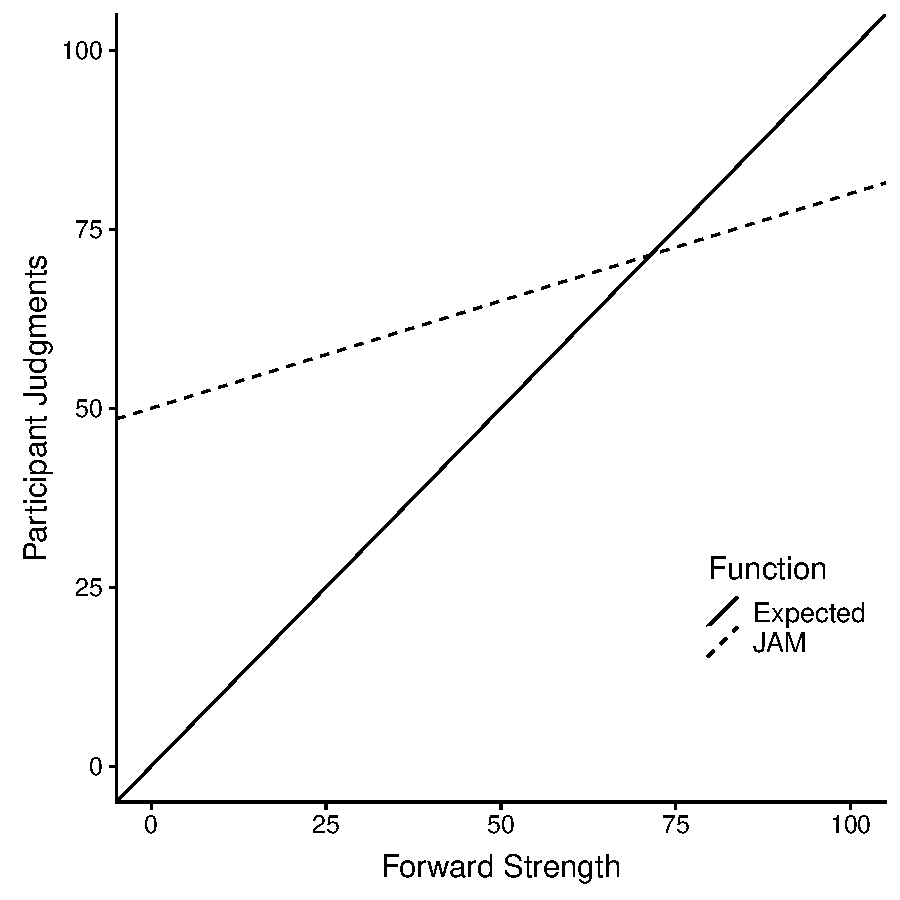
\includegraphics{max_buch_JOL_files/figure-latex/makislope-1.pdf}
\caption{\label{fig:makislope}JAM slope findings from Maki (2007a). JAM is characterized by a high intercept (between 40 and 60) and a shallow slope (between 0.20 and 0.40). The solid line shows expected results if judgment ratings are perfectly calibrated with association norms.}
\end{figure}

The discrepancy between direct association strength and JAM ratings is noteworthy because on the surface, the two tasks should each be tapping into the same concept of associative overlap. One explanation for this provided by Maki (2007a) is that judgment tasks are more easily influenced by outside factors such as the availability heuristic. Thus, it may be that the mere act of viewing the cue-target pair together at the time of judgment interferes with individuals' ability to consider other target words that are related to the cue, thereby inflating (or reducing) the perceived relatedness between the items (Maki, 2007a). Indeed, work by Nelson and Dunlosky (1991) has shown this effect when eliciting judgments of learning, as JOLs made after a delay tend to be more accurate relative to those made immediately in the presence of the studied information. Further, the influence of indirect relations on judgments has not been investigated within the context of multiple judgment types (but see De Deyne et al. (2013b) for a review of both SWOW association types within the context of semantic similarity judgments).

The present study expanded upon previous JAM studies by examining recall rates and judgment strengths for three types of judgments of relatedness (associative, semantic, and thematic; JORs) with the goal of exploring the underlying memory network that is used for each of these cognitive processes as described above. To date, no study has investigated how the three types of concept information affect these judgment and recall processes within the context of one unified study. Thus, the ensuing JOR task is a direct extension of Maki's (2007a) JAM task. As such, we tested four hypotheses, which were based upon previous research on JAM and semantic memory models.

First, we sought to expand upon previous Maki (2007a), Maki (2007b), Buchanan (2010), and Valentine and Buchanan (2013) research by using an extended JAM task that included three types of judgments within one experiment (i.e., associative, semantic, and thematic judgments), while replicating JAM bias and sensitivity findings (Hypothesis 1). Because the judgment task we employ is an extended JAM task that also includes semantic and thematic judgments, we subsequently refer to all judgment tasks as a judgment of relatedness task (JOR), regardless of which type of judgment is being elicited. We used the SWOW norms, calculating direct and indirect relations to best capture the continuum of similarity between concepts. These values were used to predict each type of JOR, and we calculated average slope and intercept values for each participant. We expected to find slope and intercept values that were significantly different from zero. Though the three types of word relations are distinct from one another, we should expect to find slopes and intercepts for semantic and thematic JORs to be within the range of previous JAM findings if these memory systems are interconnected. We also examined the frequency of each predictor being the strongest variable to predict an individual judgment condition. Thus, we are interested in exploring whether judgment findings replicate across each judgment type while using the new measurement variables available through SWOW (rather than each individually, as tested in previous JOL and JAM publications), which expands our knowledge on how the judgment process taps into the underlying memory network.

Next, we explored the predictions from semantic network models that the relation between associations and semantics would be interconnected by nature (i.e., both types of knowledge closely linked in memory). Therefore, we expected to find an interaction between direct and indirect association norms when predicting JORs. We used multilevel modeling to examine the interaction of these norms in relation to participant judgments (Hypothesis 2).

We then extended these analyses to include recall as the dependent variable of interest (Hypothesis 3). We tested for the interaction of database norms in predicting recall by using a multilevel logistic regression, while controlling for judgment conditions and rating. We expected to find that database norms would show differences in recall based on the levels of other variables (the interaction would be significant), and that ratings would also positively predict recall (i.e., words that participants thought were more related would be remembered better). Because judgment making and recall are different cognitive processes, we used this hypothesis to examine how the interactive structure of memory networks may differ based on task.

Finally, we examined if the judgment slopes from Hypothesis 1 would be predictive of recall (Hypothesis 4). Whereas the recall model used to test our third hypothesis examined the direct relationship of word relatedness on recall, the goal of this analysis was to explore whether participant sensitivity to word relatedness could also be used to predict recall. For this analysis, we used a multilevel logistic regression to control for multiple judgment slope conditions. This hypothesis combined both cognitive processes into one analysis so as to explore how judgment ability (i.e., slopes) would impact the memory process.

\hypertarget{method}{%
\section{Method}\label{method}}

\hypertarget{participants}{%
\subsection{Participants}\label{participants}}

A power analysis was conducted using the \emph{simR} package in \emph{R} (Green \& MacLeod, 2016). This package uses simulations to generate power estimates for mixed linear models created from the \emph{lme4} package in \emph{R} (Bates, Mächler, Bolker, \& Walker, 2015). The results of this analyses suggested a minimum of 35 participants would be required to detect an effect. However, because power often tends to be underestimated, we extended participant recruitment as funding permitted. The data in this experiment were collected in two waves of recruiting from Amazon's Mechanical Turk, which is a website that allows individuals to host projects and connects them with a large pool of respondents who complete them for small amounts of money (Buhrmester, Kwang, \& Gosling, 2011). In the first wave, a total of 112 participants were recruited, and in the second wave, 221 participants were recruited. Participant responses were screened for a basic understanding of the study's instructions. Responses were rejected for participants who entered related words when numerical judgment responses were required and for participants who responded to the cue words during the recall phase with sentences or phrases instead of individual words. Those that completed the study correctly were compensated \$1.00 for their participation in wave one, and \$2.00 for their participation in wave two. The second wave of participants was sponsored by graduate thesis funding provided by the Missouri State University Graduate College.

\hypertarget{materials}{%
\subsection{Materials}\label{materials}}

The stimuli used were 126 word pairs of varying relatedness, which were derived from the Buchanan et al. (2013) word norm database and website. These pairs were evenly split into sixty-three pairs for wave one and wave two of the study. Pairs were originally selected by using forward strength (FSG; Nelson et al., 2004), semantic feature overlap cosine values (COS) from Buchanan et al. (2013), and Latent Semantic Analysis cosine values (Landauer \& Dumais, 1997; Landauer, Foltz, \& Laham, 1998) based on previous research on how word pair psycholinguistic variables overlap (Maki \& Buchanan, 2008). The selected stimuli included a range of values for each variable. Table \ref{tab:stim-table} displays descriptive statistics for the stimuli pairs. A complete list of stimuli can be found at \url{http://osf.io/y8h7v}.

The stimuli were arranged into three blocks for each judgment condition described below wherein each block contained 21 word pairs. Due to limitations of the available stimuli, blocks were structured so that each one contained seven word pairs of low (0-.33), medium (.34-.66), and high (.67-1.00) COS relatedness. Pairs with low, medium, and high FSG and LSA were then selected, when available. Given the measurement questions raised in the introduction, the direct association from the SWOW norms will be used as the measure of first order association. Based on De Deyne et al. (2013a)'s work on continuous association, the response set from all three responses were used. The direct association provided in these norms is calculated as the number of participants who provided the target to the cue divided by the number of possible answers (i.e., participants \(\times\) responses). This calculation, therefore, has an upper limit of approximately \textasciitilde{}33\%, even if every participant listed a target word to a cue. The JOR task assumes the range of direct association is 0 to 100 (or 0-1 proportion), and the SWOW direct association (DA) was normalized using:

\[\frac{DA - Min(DA)} {Max(DA) - Min(DA)}\]

Indirect association (IA) was calculated by comparing the distribution of responses for each concept. Therefore, if the concepts were \emph{bird} and \emph{feather}, the two association sets were combined and the cosine between the response frequencies was calculated. Cosine indicates a measure of overlap in the response distributions, where 0 indicates no overlapping responses, while 1 indicates perfectly overlapping response frequencies (see Buchanan et al., 2019 for more on cosine feature overlap). DA and IA averages are provided in Table \ref{tab:stim-table}. The study was built online using Qualtrics, and three surveys were created to counter-balance the order in which judgment conditions appeared. Each word pair appeared counter-balanced across each judgment condition, and stimuli were randomized within each block.

\begin{table}[t]

\caption{\label{tab:stim-table}Summary Statistics for Stimuli}
\centering
\begin{tabular}{llll}
\toprule
\multicolumn{1}{c}{ } & \multicolumn{3}{c}{Semantic Feature Overlap COS} \\
\cmidrule(l{3pt}r{3pt}){2-4}
Variable & Low & Average & High\\
\midrule
Semantic Feature Overlap COS & .09 (.10) & .45 (.09) & .75 (.05)\\
Forward Strength FSG & .08 (.11) & .15 (.17) & .19 (.24)\\
Latent Semantic Analysis LSA & .25 (.17) & .39 (.18) & .47 (.18)\\
Direct Association & .12 (.16) & .23 (.23) & .27 (.29)\\
Indirect Association & .10 (.14) & .25 (.17) & .39 (.18)\\
\bottomrule
\multicolumn{4}{l}{\textsuperscript{} $Note$. Standard deviation values are in parentheses.}\\
\end{tabular}
\end{table}

\hypertarget{procedure}{%
\subsection{Procedure}\label{procedure}}

The present study was divided into three phases. In the first phase, JORs were elicited by presenting participants with word pairs and asking them to make judgments of how related they believed the words in each pair to be. This judgment phase consisted of three blocks of 21 word pairs which corresponded to one of three types of described word pair relationships: associative, semantic, or thematic. Each block was preceded by a set of instructions explaining one of the three types of relationships, and participants were provided with examples which illustrated the type of relationship to be judged. Participants were then presented with the word pairs to be judged. The associative block began by explaining associative memory and the role of free association tasks. Participants were provided with examples of both strong and weak associates. For example, \emph{lost} and \emph{found} were presented as an example of a strongly associated pair, while \emph{article} was paired with \emph{newspaper}, \emph{the}, and \emph{clothing} to illustrate that words can have many weak associates. The semantic judgment block provided participants with a brief overview of how words are related by meaning and showed examples of concepts with both high and low feature overlap. \emph{Tortoise} and \emph{turtle} were provided as an example of two concepts with significant overlap. Other examples were then provided to illustrate concepts with little or no overlap. For the thematic judgments, participants were provided with an explanation of thematic relatedness. \emph{Tree} is explained to be related to \emph{leaf}, \emph{fruit}, and \emph{branch}, but not \emph{computer}. For each judgment condition, participants were then given three concepts (\emph{lost}, \emph{old}, \emph{article}) and were asked to come up with words that they felt were related to that type of relation.

After viewing the examples at the start of the block, participants completed the JOR task. Each block contained a set of instructions which were contingent upon the type of JOR being elicited. For example, instructions in the associative block asked participants to estimate how many individuals out of 100 they expect would respond to the cue word with a given target, instructions for semantic JORs asked participants to indicate the percent of features shared between two concepts, and instructions for the thematic JOR task asked participants to base ratings on how likely to words would be used together in the same story. The complete experiment can be found at \url{http://osf.io/y8h7v}, which contains the exact instructions given to participants for each block and displays the structure of the study. All instructions were modeled after Buchanan (2010) and Valentine and Buchanan (2013).

In accordance with previous work on JOLs and JAM, participants made JOR ratings using a scale of zero to one hundred, with zero indicating no relationship, and one hundred indicating a perfect relationship. Participants typed their responses into the survey. Once finished, participants then completed the remaining judgment blocks in the same manner. Each subsequent judgment block changed the type of JOR being made. Three versions of the study were created, which counter-balanced the order in which the judgment blocks appeared, and participants were randomly assigned to a survey version. This resulted in each word pair receiving a relatedness judgment on each of the three types relationships.

After completing the judgment phase, participants were then presented with a short distractor task to account for recency effects. In this section, participants were presented with a randomized list of the fifty U.S. states and were asked to arrange them in alphabetical order. This task was timed to last two minutes. Once time had elapsed, participants automatically progressed to the final phase, which consisted of a cued-recall task. Participants were presented with each of the sixty-three cue words from the judgment phase and were asked to complete each word pair by responding with the correct target word. Participants were informed that they would not be penalized for guessing. The cued-recall task included all stimuli in a random order.

\hypertarget{results}{%
\section{Results}\label{results}}

\hypertarget{data-processing-and-descriptive-statistics}{%
\subsection{Data Processing and Descriptive Statistics}\label{data-processing-and-descriptive-statistics}}

First, the results from the recall phase of the study were coded as zero for incorrect responses, one for correct responses, and NA for participants who did not complete the recall section (all or nearly all responses were blank). All word responses to judgment items were deleted and set to missing data\footnote{The final dataset was created by splitting the initial data file into six sections (one for each of the three experimental blocks and their corresponding recall scores). Each section was individually melted using the \emph{reshape} package in \emph{R} (Wickham, 2007) and was written as a csv file. The six output files were then combined to form the final dataset. Code is available on our OSF page embedded inline with the manuscript in an \emph{R} markdown document written with the \emph{papaja} package (Aust \& Barth, 2017).}. With 333 participants, the dataset in long format (i.e., each judgment and recall on their own row) included 20979 rows of potential data (i.e., 333 participants \(\times\) 63 JORs). 15 out of range JOR data points (\textgreater{} 100) were corrected to NA. Missing data for JORs or recall were then excluded from the analyses, which included word responses to judgment items (i.e., responding with \emph{cat} instead of a number when prompted to provide a JOR). These items usually excluded a participant from receiving Amazon Mechanical Turk payment, but were included in the datasets found online. In total, 2266 data points were excluded (679 JOR only, 1019 recall only, 568 both), leading to a final \emph{N} of 18713 observations. Recall and JOR values were then screened for outliers using Mahalanobis distance at \emph{p} \textless{} .001, and no outliers were detected (Tabachnick \& Fidell, 2012). To screen for multicollinearity, we examined correlations between judgment items, DA, and IA. The correlations between judged values, recall, direct and indirect associations were all \emph{r}s \textless{} .26. These correlations were similar regardless of judgment condition.

The mean JOR for the associative condition (\emph{M} = 59.40, \emph{SD} = 29.52) was lower than the semantic (\emph{M} = 64.15, \emph{SD} = 29.74) and thematic (\emph{M} = 69.50, \emph{SD} = 28.20) conditions. A multilevel model was examined to determine if these JOR values were significantly different using participants as a random factor. Multilevel models were used to retain all data points (rather than averaging over items and conditions) while controlling for correlated error due to participants, which makes these models advantageous for multiway repeated measures designs (Gelman, 2006). Associative judgments were lower than both semantic (\emph{t}(19407) = 10.40, \emph{p} \textless{} .001), and thematic judgments (\emph{t}(19407) = 22.25, \emph{p} \textless{} .001). Semantic judgments in turn were lower than thematic judgments (\emph{t}(19407) = 11.85, \emph{p} \textless{} .001).

Recall averaged around 60\% for all three conditions: associative \emph{M} = 59.04, \emph{SD} = 49.18; semantic \emph{M} = 62.57, \emph{SD} = 48.40; thematic \emph{M} = 60.12, \emph{SD} = 48.97. A separate multilevel model indicated that associative recall was lower than semantic recall (\emph{t}(19064) = 4.63, \emph{p} \textless{} .001), but not thematic recall (\emph{t}(19064) = 1.37, \emph{p} = .169). Semantic recall scores were higher than thematic recall scores (\emph{t}(19064) = -3.25, \emph{p} = .001).

\hypertarget{jam-slope-bias-and-sensitivity}{%
\subsection{JAM Slope Bias and Sensitivity}\label{jam-slope-bias-and-sensitivity}}

\begin{table}[tbp]
\begin{center}
\begin{threeparttable}
\caption{\label{tab:hyp1-table1}Summary Statistics for Hypothesis 1 t-Tests}
\begin{tabular}{lccccccc}
\toprule
Judgment - Variable & $M$ & $SD$ & $t$ & $df$ & $p$ & $d$ & $95\% CI$\\
\midrule
Associative Intercept & .52 & .20 & 45.90 & 311 & < .001 & 2.60 & 2.36 - 2.83\\
Associative Direct Association & .33 & .30 & 19.27 & 311 & < .001 & 1.09 & 0.95 - 1.23\\
Associative Indirect Association & .03 & .29 & 1.62 & 311 & .105 & 0.09 & -0.02 - 0.20\\
Semantic Intercept & .52 & .21 & 44.64 & 312 & < .001 & 2.52 & 2.29 - 2.75\\
Semantic Direct Association & .31 & .30 & 18.47 & 312 & < .001 & 1.04 & 0.91 - 1.18\\
Semantic Indirect Association & .24 & .32 & 13.31 & 312 & < .001 & 0.75 & 0.63 - 0.88\\
Thematic Intercept & .61 & .18 & 59.25 & 315 & < .001 & 3.33 & 3.05 - 3.61\\
Thematic Direct Association & .28 & .27 & 18.54 & 315 & < .001 & 1.04 & 0.91 - 1.18\\
Thematic Indirect Association & .14 & .28 & 8.65 & 315 & < .001 & 0.49 & 0.37 - 0.60\\
\bottomrule
\addlinespace
\end{tabular}
\begin{tablenotes}[para]
\normalsize{\textit{Note.} Confidence interval for $d$ was calculated using the non-central $t$-distribution. Hypothesis 1 investigated if bias and sensitivity findings replicated in association and extended to semantic and thematic judgment conditions.}
\end{tablenotes}
\end{threeparttable}
\end{center}
\end{table}

First, we sought to replicate bias and sensitivity findings from previous research while expanding the JAM function to include judgments based on three types of memory. DA and IA were used to predict each type of relatedness judgment. JOR values were divided by 100, so as to place them on the same scale as the direct and indirect association measures. Slopes and intercepts were then calculated for each participant's ratings for each of the three JOR conditions, as long as they contained at least nine data points out of the twenty-one that were possible. Single sample \emph{t}-tests were then conducted to test if slope and intercept values significantly differed from zero. See Table \ref{tab:hyp1-table1} for means and standard deviations. Slopes were then compared to the JAM function, which is characterized by high intercepts (between 40 and 60 on a 100 point scale) and shallow slopes (between 20 and 40). Because of the scaling of our data, to replicate this function, we should expect to find intercepts ranging from .40 to .60 and slopes in the range of .20 to .40. Intercepts for associative, semantic, and thematic JORs were each significant, and all fell within or near the expected range. Overall, thematic JORs had the highest intercept at .61, while JORs elicited in the semantic and associative conditions had the lower intercepts at .52 each.

The JAM slope was successfully replicated for DA in all three judgment conditions, with slopes falling in the expected range of .20 to .40. For associative judgments, the indirect relation - which is thought to be representative of semantic relatedness - did not predict judgments \(M_b\) = .03. In the thematic judgment condition, the indirect values were positive \(M_b\) = .14, indicating a contribution of both direct \(M_b\) = .28 and indirect values to the judgments, which were described as being a mix of both relation types. Last, the semantic judgment condition showed that both direct \(M_b\) = .31 and indirect \(M_b\) = .24 relations were important (as this judgment type had the highest indirect contribution of the three conditions), indicating that differences in the focus of judgments tap different relations to meet task demands. Overall, JAM slopes were successfully replicated in each JOR condition, and the high intercepts and shallow slopes present across conditions were indicative of overconfidence and insensitivity in participant JORs.

Additionally, we examined the frequency that each predictor variable was the strongest predictor for each of the three JOR conditions. For the associative condition, the direct association was the strongest predictor for 67.3\% of the participants. This distinction was less pronounced when examining the semantic and thematic JOR conditions. In the semantic condition, DA was 52.1\% of participants, and in the thematic condition, DA was 54.1\% of participants. These results mirror the slope values, such that direct association is strongest when participants are asked to judge associative relations, while a more even split between direct and indirect predictors was found when participants were asked to consider semantic and thematic relations.

\hypertarget{interaction-between-relation-when-predicting-judgments-of-relatedness}{%
\subsection{Interaction between Relation when Predicting Judgments of Relatedness}\label{interaction-between-relation-when-predicting-judgments-of-relatedness}}

\begin{table}[tbp]
\begin{center}
\begin{threeparttable}
\caption{\label{tab:hyp2-table}MLM Statistics for Hypothesis 2}
\begin{tabular}{lcccc}
\toprule
Statistic & \multicolumn{1}{c}{Coefficient} & \multicolumn{1}{c}{$SE$} & \multicolumn{1}{c}{$t$} & \multicolumn{1}{c}{$p$}\\
\midrule
Intercept & 0.59 & 0.01 & 77.47 & < .001\\
Semantic Judgment & 0.05 & 0.00 & 10.73 & < .001\\
Thematic Judgment & 0.10 & 0.00 & 23.11 & < .001\\
Z Direct Association & 0.29 & 0.01 & 38.98 & < .001\\
Z Indirect Association & 0.14 & 0.01 & 15.92 & < .001\\
Z Interaction & -0.19 & 0.05 & -3.86 & < .001\\
Z Direct Association Low & 0.33 & 0.01 & 26.40 & < .001\\
Z Direct Association High & 0.25 & 0.01 & 20.58 & < .001\\
\bottomrule
\addlinespace
\end{tabular}
\begin{tablenotes}[para]
\normalsize{\textit{Note.} Direct and indirect association were mean centered. The table shows results from the second hypothesis wherein an interaction between direct and indirect association was investigated predicting judgment score. $df$ = 19404}
\end{tablenotes}
\end{threeparttable}
\end{center}
\end{table}

\begin{figure}
\centering
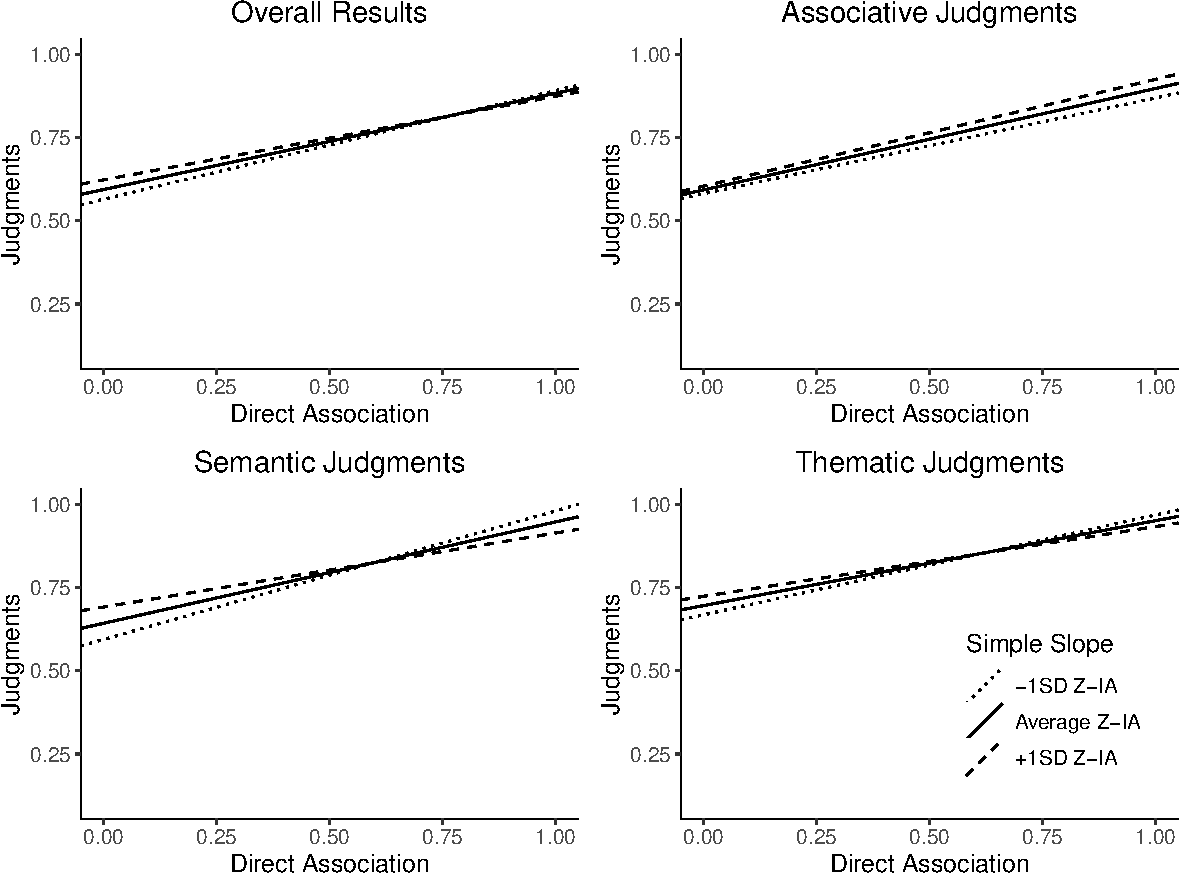
\includegraphics{max_buch_JOL_files/figure-latex/hyp2graph-1.pdf}
\caption{\label{fig:hyp2graph}Simple slopes graph displaying the slope of direct association when predicting JORs at low, average, and high indirect association. All variables were mean centered. The top left panel displays overall analysis adjusting for condition. The other three panels indicate associative (no interaction), semantic, and thematic judgments individually.}
\end{figure}

Next, we sought to test the interactive relationship between associative and semantic overlap. If this interactive relationship exists, a statistical interaction should be detected between the database norms when predicting performance on the judgment task. As such, the goal of next analysis was to test for this interaction between direct and indirect association when predicting participant JORs. First, the database norms were mean centered to aid in interpretation. The \emph{nlme} package and \emph{lme} function were used to calculate these analyses (Pinheiro, Bates, Debroy, Sarkar, \& R Core Team, 2017). A maximum likelihood multilevel model was used to test for the interaction between DA and IA when predicting JOR values, with participant number used as the random intercept factor. The type of JOR being elicited was controlled for so as to better assess the impact of each word overlap measure regardless of JOR condition. This analysis resulted in a significant interaction between DA and IA (\(\beta\) = -0.19, \emph{p} \textless{} .001), which is examined below in a simple slopes analysis. Table \ref{tab:hyp2-table} includes values for main effects, two-way interaction, and the simple slopes.

To investigate this interaction, simple slopes were calculated for low, average, and high levels of indirect association. This variable was chosen to show the effects of direct associations across levels of indirect association. At low levels of indirect relation (and thus low levels of the semantic network), we found the largest \(\beta\) for direct association, 0.33. As indirect relation increased, we found decreasing predictiveness of direct relation, average direct \(\beta\) = 0.29, and high direct \(\beta\) = 0.25. Figure \ref{fig:hyp2graph} displays the two-way interaction with this seesaw type effect, indicating that higher semantic network relation results in lower usefulness of direct associative relation. Further, we then split the data by judgment type to visualize the interaction in each condition, as Hypothesis 1 indicated some task demand characteristics. The results are consistent in semantic and thematic judgments (lower two panels), while no interaction was found in the associative judgment condition (top right panel). The complete table of predictors for these analyses can be found at \url{http://osf.io/y8h7v}.

\hypertarget{interaction-between-relation-when-predicting-recall}{%
\subsection{Interaction between Relation when Predicting Recall}\label{interaction-between-relation-when-predicting-recall}}

\begin{table}[tbp]
\begin{center}
\begin{threeparttable}
\caption{\label{tab:hyp3-table}MLM Statistics for Hypothesis 3}
\begin{tabular}{lcccc}
\toprule
Statistic & \multicolumn{1}{c}{Coefficient} & \multicolumn{1}{c}{$SE$} & \multicolumn{1}{c}{$Z$} & \multicolumn{1}{c}{$p$}\\
\midrule
Intercept & 0.42 & 0.08 & 5.09 & < .001\\
Semantic Judgment & 0.18 & 0.04 & 4.38 & < .001\\
Thematic Judgment & 0.05 & 0.04 & 1.10 & .270\\
Judged Value & 0.04 & 0.07 & 0.66 & .512\\
Z Direct Association & 1.63 & 0.08 & 20.32 & < .001\\
Z Indirect Association & 0.32 & 0.09 & 3.71 & < .001\\
Z Interaction & -1.30 & 0.49 & -2.67 & .008\\
Z Direct Association Low & 1.90 & 0.13 & 14.58 & < .001\\
Z Direct Association High & 1.37 & 0.12 & 11.09 & < .001\\
\bottomrule
\addlinespace
\end{tabular}
\begin{tablenotes}[para]
\normalsize{\textit{Note.} Direct and indirect association were mean centered. The table shows results from the third hypothesis extending the interaction between direct and indirect associations to recall for words.}
\end{tablenotes}
\end{threeparttable}
\end{center}
\end{table}

\begin{figure}
\centering
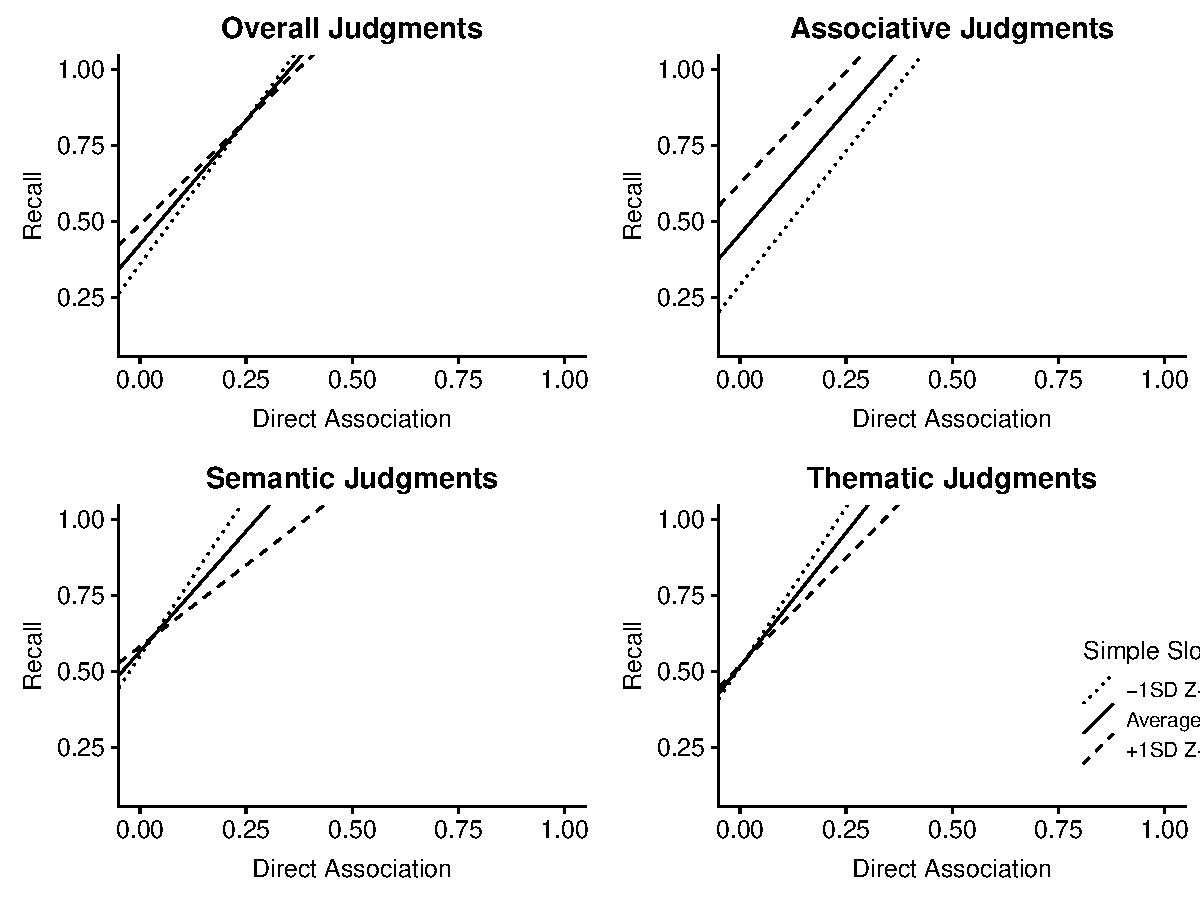
\includegraphics{max_buch_JOL_files/figure-latex/hyp3graph-1.pdf}
\caption{\label{fig:hyp3graph}Simple slopes graph displaying the slope of direct association when predicting recall at low, average, and high indirect association. All variables were mean centered. The top left panel displays overall analysis adjusting for condition. The other three panels indicate associative (no interaction), semantic, and thematic judgments individually.}
\end{figure}

Given the results of Hypothesis 2, we then sought to extend the analysis to participant recall scores. A multilevel logistic regression was used with the \emph{lme4} package and \emph{glmer()} function (Bates et al., 2015), testing the interaction between DA and IA when predicting participant recall. As with the previous hypothesis, we controlled for JOR condition and, additionally, covaried JOR ratings. Participants were used as a random intercept factor. Judged values were not a significant predictor of recall, (\(\beta\) = 0.04, \emph{p} = .512). A significant interaction was detected between direct and indirect relations (\(\beta\) = -1.30, \emph{p} = .008). See Table \ref{tab:hyp3-table} for main effects, interaction, and simple slopes.

The same moderation process used in Hypothesis 2 was then repeated, with simple slopes calculated at low, average, and high levels of indirect association. The same pattern of results emerged where low levels of indirect association resulted in the largest contribution of direct association \(\beta\) = 1.90. As indirect association increased, direct association coefficients decreased, average direct \(\beta\) = 1.63, and high direct \(\beta\) = 1.37. Thus, the cognitive processes of recall and judgment appear to operate similarly on the memory network. Again, we analyzed these results separately for each condition, as shown in Figure \ref{fig:hyp3graph}. The results indicated that there was not an interaction for associative judgments, but semantic and thematic judgments included the direct-indirect association interaction as described above. These results mirror those found in for judgments, and the entire set of predictors can be found online.

\hypertarget{predicting-recall-with-jam-slopes}{%
\subsection{Predicting Recall with JAM Slopes}\label{predicting-recall-with-jam-slopes}}

\begin{table}[tbp]
\begin{center}
\begin{threeparttable}
\caption{\label{tab:hyp4-table}MLM Statistics for Hypothesis 4}
\begin{tabular}{lcccc}
\toprule
Judgment - Variable & \multicolumn{1}{c}{$b$} & \multicolumn{1}{c}{$SE$} & \multicolumn{1}{c}{$z$} & \multicolumn{1}{c}{$p$}\\
\midrule
(Intercept) & -0.11 & 0.27 & -0.40 & .690\\
Associative Direct Association & 1.17 & 0.26 & 4.54 & < .001\\
Associative Indirect Association & -0.10 & 0.23 & -0.42 & .673\\
Associative Intercept & 0.49 & 0.39 & 1.24 & .214\\
(Intercept) & -1.16 & 0.31 & -3.71 & < .001\\
Semantic Direct Association & 1.31 & 0.25 & 5.19 & < .001\\
Semantic Indirect Association & 1.27 & 0.23 & 5.50 & < .001\\
Semantic Intercept & 1.80 & 0.43 & 4.20 & < .001\\
(Intercept) & -1.00 & 0.32 & -3.15 & .002\\
Thematic Direct Association & 1.09 & 0.27 & 4.11 & < .001\\
Thematic  Indirect Association & 1.05 & 0.25 & 4.17 & < .001\\
Thematic Intercept & 1.74 & 0.42 & 4.09 & < .001\\
\bottomrule
\addlinespace
\end{tabular}
\begin{tablenotes}[para]
\normalsize{\textit{Note.} This hypothesis investigated how each judgment's original bias intercept score and sensitivity slope score would predict the corresponding judgment condition. (Intercept) is the intercept for the overall model, while the Judgment Intercepts are the bias scores for each participant from Hypothesis 1.}
\end{tablenotes}
\end{threeparttable}
\end{center}
\end{table}

In our fourth and final hypothesis, we investigated whether the JOR slopes and intercepts obtained in Hypothesis 1 would be predictive of recall ability. Whereas Hypothesis 3 indicated that word relatedness was directly related to recall performance, this hypothesis instead looked at whether or not participants' sensitivity and bias to word relatedness could be used as a predictor of recall (Maki, 2007b). This analysis was conducted with a multilevel logistic regression, as described in Hypothesis 3, where each direct and indirect slope and intercept was used as a predictor of recall using participant number as a random intercept factor. These analyses were separated by judgment condition, so that each set of JOR slopes and intercepts was used to predict recall. The separation controlled for the number of variables in the equation, as all slopes and intercepts would have resulted in overfitting. These values were obtained from Hypothesis 1, where each participant's individual slopes and intercepts were calculated for associative, semantic, and thematic JOR conditions. Table \ref{tab:hyp1-table1} shows average slopes and intercepts for recall for each of the three types of memory, and Table \ref{tab:hyp4-table} portrays the regression coefficients and statistics.

In the associative condition, the direct association slope significantly predicted recall (\emph{b} = 1.17, \emph{p} \textless{} .001), while the indirect association did not predict recall (\emph{b} = -0.10, \emph{p} = .673). However, in both of the semantic and thematic conditions, the direct and indirect relations are both predictors, along with the intercepts (see Table \ref{tab:hyp4-table}). In each of these judgment conditions, the direct and indirect association predictors have similar coefficients, showing equal weight in the prediction of recall. Therefore, higher levels of sensitivity in judgments contribute to higher recall, and higher bias in judgments also leads to more recall. These results mimic the results from across our hypotheses, wherein the associative condition was predicted by direct associations, while the semantic and thematic conditions were predicted by both direct and indirect associations. This analysis indicated the extent to which the cognitive processes are related to each other as part of the memory network (i.e., judgment sensitivity predicting recall), furthering the previous two analyses, which illustrated the nature of those cognitive processes' relationship with the underlying memory network.

\hypertarget{discussion}{%
\section{Discussion}\label{discussion}}

This study investigated the relationship between direct (associative) and indirect (semantic) relations and their effect on participant JORs and recall performance through the testing of four hypotheses. In our first hypothesis, we show that bias and sensitivity findings first proposed by Maki (2007a) successfully replicated in all three judgment conditions. Participants displayed high intercepts and shallow slopes, suggesting overconfidence in judgment making and an insensitivity to changes in strength between pairs. Additionally, when looking at the frequency that each predictor was the strongest in making JORs, direct association was the strongest predictor for the associative condition, with a nearly even split between direct and indirect association for the semantic and thematic conditions. The observation that direct association was the strongest predictor of both judgments and recall within the associative condition and that the indirect association was strongest for the semantic and thematic conditions is not surprising. Direct associations are designed to capture the associative overlap shared between word pairs whereas indirect associations are thought to tap into elements of the overall semantic network and represent similarities in meaning rather than cue-target probabilities. Therefore, these results appear to reflect the task demands for each judgment condition. This finding may also be comparable to results in the semantic priming literature, wherein direct and indirectly related pairs show different priming effects (Lerner, Bentin, \& Shriki, 2012), often modulated by task (Jones, 2010, 2012), and recognition has also been shown to be influenced by indirect relations (Huff, Coane, Hutchison, Grasser, \& Blais, 2012; Huff \& Hutchison, 2011).

Finally, in contrast to the study conducted by De Deyne et al. (2013a), we found bias in judgments for pairs with no direct relation across each of the three judgment conditions (average judgment = 50.36); however, these findings should be viewed cautiously as our stimuli contained only 5 item pairs that had no direct association. The SWOW norms size and construction lessens the measurement bias in the data, and these results support that some overestimation bias likely exists beyond potential measurement bias, especially in line with the traditional judgments of learning literature.

Our second hypothesis examined if there was an interaction between direct and indirect association when predicting participant JORs. The interaction was present as a seesaw effect wherein increasing levels of indirect association lead to decreasing predictiveness of direct association. Therefore, as semantic connections become stronger in the memory network, the direct associative connections become less useful for judgments. This finding was extended to recall in our third hypothesis, supporting the notion that recall and judgment cognitive processes draw in similar ways on the memory network.

Finally, our fourth hypothesis used the JOR slopes and intercepts calculated in Hypothesis 1 to investigate whether participants' bias and sensitivity to word relatedness could be used to predict recall. For the associative condition, the only the direct association slope significantly predicted recall. In the semantic and thematic conditions, both direct and indirect associations, along with their intercepts, predicted recall. These results mirror results from Hypothesis 1 suggesting that task demands from the judgment instructions carry over into recall processes. For direct association, increasing sensitivity to the relation between pairs lead to increasing likelihood of memory, which is not surprising. Indirect association also showed this effect, that stronger indirect sensitivity to word pair relation also increased memory in the thematic and semantic judgment conditions, similar to indirect memory results from Huff and Hutchison (2011) and Huff et al. (2012). The intercepts or bias estimates from the first hypothesis indicated that increasing participant overestimation of weakly related pairs also predicted increased recall. Potentially, this result can be viewed as self-fulfilling, the more related participants thought the weakly related word pairs were, they more likely they were to remember them.

Overall, our findings indicated the degree to which the processing of direct and indirect word-pair network information impacts retrieval and judgment making tasks. Previous research has shown the effects of direct associations on priming (Buchanan, 2010; Hutchison, 2003), cued-recall (Nelson, Bennett, \& Leibert, 1997; Nelson, Zhang, \& McKinney, 2001), judgments of associative memory (De Deyne et al., 2013a; Maki, 2007b, 2007a; Valentine \& Buchanan, 2013) and response latencies (De Deyne et al., 2013b) to name a few. Our results suggest a competitive network based on task-demand. When instructed to focus on associative relatedness, direct association strength was a strong (and often the only) predictor of judgment or recall. When directed to focus on semantic or thematic type relations, both indirect and direct association play a role in judgments and recall. Further, this effect was interactive, wherein different levels of indirect semantic strength lead to different activation of the direct associative network. As indirect strength increases, the effect of direct strength decreases, albeit does not completely diminish.

Finally, future studies may wish to consider the effect of each concept's linguistic features (frequency, orthography, part of speech, etc.), as these properties have been shown to influence judgments and recall. The type, or ontology (Wu \& Barsalou, 2009), of the relation may provide clues as to judgments and recall. De Deyne, Navarro, Perfors, and Storms (2016) illustrated how a spreading activation model with random walks can account for participant's understanding of similarity, even when word-pair relation would be considered very weak. These models provide future avenues for application to judgment and recall processes, as we have shown they are related to the same direct and indirect network of association.

\hypertarget{compliance-with-ethical-standards}{%
\subsection{Compliance with Ethical Standards}\label{compliance-with-ethical-standards}}

The authors declare that they have no conflict of interest. The study was approved by the Institutional Review Board at Missouri State University. Participants filled out an informed consent at the beginning of the study, after accepting the HIT on Mechanical Turk. The complete study with consent form can be found on our OSF page: \url{http://osf.io/y8h7v}.

\newpage

\hypertarget{references}{%
\section{References}\label{references}}

\setlength{\parindent}{-0.5in}
\setlength{\leftskip}{0.5in}

\hypertarget{refs}{}
\leavevmode\hypertarget{ref-Aust2017}{}%
Aust, F., \& Barth, M. (2017). papaja: Create APA manuscripts with R Markdown. Retrieved from \url{https://github.com/crsh/papaja}

\leavevmode\hypertarget{ref-Bates2015}{}%
Bates, D., Mächler, M., Bolker, B., \& Walker, S. (2015). Fitting linear mixed-effects models using lme4. \emph{Journal of Statistical Software}, \emph{67}(1), 1--48. doi:\href{https://doi.org/10.18637/jss.v067.i01}{10.18637/jss.v067.i01}

\leavevmode\hypertarget{ref-Buchanan2010}{}%
Buchanan, E. M. (2010). Access into memory: Differences in judgments and priming for semantic and associative memory. \emph{Journal of Scientific Psychology}, \emph{March}, 1--8.

\leavevmode\hypertarget{ref-Buchanan2013}{}%
Buchanan, E. M., Holmes, J. L., Teasley, M. L., \& Hutchison, K. A. (2013). English semantic word-pair norms and a searchable Web portal for experimental stimulus creation. \emph{Behavior Research Methods}, \emph{45}(3), 746--757. doi:\href{https://doi.org/10.3758/s13428-012-0284-z}{10.3758/s13428-012-0284-z}

\leavevmode\hypertarget{ref-Buchanan2019}{}%
Buchanan, E. M., Valentine, K. D., \& Maxwell, N. P. (2019). English semantic feature production norms: An extended database of 4436 concepts. \emph{Behavior Research Methods}, \emph{51}(4), 1849--1863. doi:\href{https://doi.org/10.3758/s13428-019-01243-z}{10.3758/s13428-019-01243-z}

\leavevmode\hypertarget{ref-Buhrmester2011}{}%
Buhrmester, M., Kwang, T., \& Gosling, S. D. (2011). Amazon's Mechanical Turk. \emph{Perspectives on Psychological Science}, \emph{6}(1), 3--5. doi:\href{https://doi.org/10.1177/1745691610393980}{10.1177/1745691610393980}

\leavevmode\hypertarget{ref-Chow2014}{}%
Chow, B. W.-Y. (2014). The differential roles of paired associate learning in Chinese and English word reading abilities in bilingual children. \emph{Reading and Writing}, \emph{27}(9), 1657--1672. doi:\href{https://doi.org/10.1007/s11145-014-9514-3}{10.1007/s11145-014-9514-3}

\leavevmode\hypertarget{ref-DeDeyne2018}{}%
De Deyne, S., Navarro, D. J., Perfors, A., Brysbaert, M., \& Storms, G. (2019). The ``Small World of Words'' English word association norms for over 12,000 cue words. \emph{Behavior Research Methods}, \emph{51}(3), 987--1006. doi:\href{https://doi.org/10.3758/s13428-018-1115-7}{10.3758/s13428-018-1115-7}

\leavevmode\hypertarget{ref-DeDeyne2016}{}%
De Deyne, S., Navarro, D. J., Perfors, A., \& Storms, G. (2016). Structure at every scale: A semantic network account of the similarities between unrelated concepts. \emph{Journal of Experimental Psychology: General}, \emph{145}(9), 1228--1254. doi:\href{https://doi.org/10.1037/xge0000192}{10.1037/xge0000192}

\leavevmode\hypertarget{ref-DeDeyne2013a}{}%
De Deyne, S., Navarro, D. J., \& Storms, G. (2013a). Associative strength and semantic activation in the mental lexicon: evidence from continued word associations. In \emph{Proceedings of the 35th annual conference of the cognitive science society} (pp. 2142--2147).

\leavevmode\hypertarget{ref-DeDeyne2013}{}%
De Deyne, S., Navarro, D. J., \& Storms, G. (2013b). Better explanations of lexical and semantic cognition using networks derived from continued rather than single-word associations. \emph{Behavior Research Methods}, \emph{45}(2), 480--498. doi:\href{https://doi.org/10.3758/s13428-012-0260-7}{10.3758/s13428-012-0260-7}

\leavevmode\hypertarget{ref-Deese1965}{}%
Deese, J. (1965). \emph{The structure of association in language and thought}. Baltimore, MD: The Johns Hopkins University Press.

\leavevmode\hypertarget{ref-Gelman2006}{}%
Gelman, A. (2006). Multilevel (hierarchical) modeling: What it can and cannot do. \emph{Technometrics}, \emph{48}(3), 432--435. doi:\href{https://doi.org/10.1198/004017005000000661}{10.1198/004017005000000661}

\leavevmode\hypertarget{ref-Green2016}{}%
Green, P., \& MacLeod, C. J. (2016). SIMR: an R package for power analysis of generalized linear mixed models by simulation. \emph{Methods in Ecology and Evolution}, \emph{7}(4), 493--498. doi:\href{https://doi.org/10.1111/2041-210X.12504}{10.1111/2041-210X.12504}

\leavevmode\hypertarget{ref-Hertzog2002}{}%
Hertzog, C., Kidder, D. P., Powell-Moman, A., \& Dunlosky, J. (2002). Aging and monitoring associative learning: Is monitoring accuracy spared or impaired? \emph{Psychology and Aging}, \emph{17}(2), 209--225. doi:\href{https://doi.org/10.1037/0882-7974.17.2.209}{10.1037/0882-7974.17.2.209}

\leavevmode\hypertarget{ref-Huff2012b}{}%
Huff, M. J., Coane, J. H., Hutchison, K. A., Grasser, E. B., \& Blais, J. E. (2012). Interpolated task effects on direct and mediated false recognition: Effects of initial recall, recognition, and the ironic effect of guessing. \emph{Journal of Experimental Psychology: Learning Memory and Cognition}, \emph{38}(6), 1720--1730. doi:\href{https://doi.org/10.1037/a0028476}{10.1037/a0028476}

\leavevmode\hypertarget{ref-Huff2011}{}%
Huff, M. J., \& Hutchison, K. A. (2011). The effects of mediated word lists on false recall and recognition. \emph{Memory \& Cognition}, \emph{39}(6), 941--953. doi:\href{https://doi.org/10.3758/s13421-011-0077-0}{10.3758/s13421-011-0077-0}

\leavevmode\hypertarget{ref-Hutchison2003}{}%
Hutchison, K. A. (2003). Is semantic priming due to association strength or feature overlap? A microanalytic review. \emph{Psychonomic Bulletin \& Review}, \emph{10}(4), 785--813. doi:\href{https://doi.org/10.3758/BF03196544}{10.3758/BF03196544}

\leavevmode\hypertarget{ref-Jones2010}{}%
Jones, L. L. (2010). Pure mediated priming: A retrospective semantic matching model. \emph{Journal of Experimental Psychology: Learning Memory and Cognition}, \emph{36}(1), 135--146. doi:\href{https://doi.org/10.1037/a0017517}{10.1037/a0017517}

\leavevmode\hypertarget{ref-Jones2012a}{}%
Jones, L. L. (2012). Prospective and retrospective processing in associative mediated priming. \emph{Journal of Memory and Language}, \emph{66}(1), 52--67. doi:\href{https://doi.org/10.1016/j.jml.2011.08.005}{10.1016/j.jml.2011.08.005}

\leavevmode\hypertarget{ref-Koriat2005}{}%
Koriat, A., \& Bjork, R. A. (2005). Illusions of competence in monitoring one's knowledge during study. \emph{Journal of Experimental Psychology: Learning, Memory, and Cognition}, \emph{31}(2), 187--194. doi:\href{https://doi.org/10.1037/0278-7393.31.2.187}{10.1037/0278-7393.31.2.187}

\leavevmode\hypertarget{ref-Landauer1997}{}%
Landauer, T. K., \& Dumais, S. T. (1997). A solution to Plato's problem: The latent semantic analysis theory of acquisition, induction, and representation of knowledge. \emph{Psychological Review}, \emph{104}(2), 211--240. doi:\href{https://doi.org/10.1037//0033-295X.104.2.211}{10.1037//0033-295X.104.2.211}

\leavevmode\hypertarget{ref-Landauer1998}{}%
Landauer, T. K., Foltz, P. W., \& Laham, D. (1998). An introduction to latent semantic analysis. \emph{Discourse Processes}, \emph{25}(2), 259--284. doi:\href{https://doi.org/10.1080/01638539809545028}{10.1080/01638539809545028}

\leavevmode\hypertarget{ref-Lerner2012}{}%
Lerner, I., Bentin, S., \& Shriki, O. (2012). Spreading activation in an attractor network with latching dynamics: Automatic semantic priming revisited. \emph{Cognitive Science}, \emph{36}(8), 1339--1382. doi:\href{https://doi.org/10.1111/cogs.12007}{10.1111/cogs.12007}

\leavevmode\hypertarget{ref-Lund1996}{}%
Lund, K., \& Burgess, C. (1996). Producing high-dimensional semantic spaces from lexical co-occurrence. \emph{Behavior Research Methods, Instruments, \& Computers}, \emph{28}(2), 203--208. doi:\href{https://doi.org/10.3758/BF03204766}{10.3758/BF03204766}

\leavevmode\hypertarget{ref-Maki2007a}{}%
Maki, W. S. (2007a). Judgments of associative memory. \emph{Cognitive Psychology}, \emph{54}(4), 319--353. doi:\href{https://doi.org/10.1016/j.cogpsych.2006.08.002}{10.1016/j.cogpsych.2006.08.002}

\leavevmode\hypertarget{ref-Maki2007}{}%
Maki, W. S. (2007b). Separating bias and sensitivity in judgments of associative memory. \emph{Journal of Experimental Psychology. Learning, Memory, and Cognition}, \emph{33}(1), 231--237. doi:\href{https://doi.org/10.1037/0278-7393.33.1.231}{10.1037/0278-7393.33.1.231}

\leavevmode\hypertarget{ref-Maki2008}{}%
Maki, W. S., \& Buchanan, E. M. (2008). Latent structure in measures of associative, semantic, and thematic knowledge. \emph{Psychonomic Bulletin \& Review}, \emph{15}(3), 598--603. doi:\href{https://doi.org/10.3758/PBR.15.3.598}{10.3758/PBR.15.3.598}

\leavevmode\hypertarget{ref-Maki2004}{}%
Maki, W. S., McKinley, L. N., \& Thompson, A. G. (2004). Semantic distance norms computed from an electronic dictionary (WordNet). \emph{Behavior Research Methods, Instruments, \& Computers}, \emph{36}(3), 421--431. doi:\href{https://doi.org/10.3758/BF03195590}{10.3758/BF03195590}

\leavevmode\hypertarget{ref-McRae2005}{}%
McRae, K., Cree, G. S., Seidenberg, M. S., \& McNorgan, C. (2005). Semantic feature production norms for a large set of living and nonliving things. \emph{Behavior Research Methods}, \emph{37}(4), 547--559. doi:\href{https://doi.org/10.3758/BF03192726}{10.3758/BF03192726}

\leavevmode\hypertarget{ref-Nelson1997}{}%
Nelson, D. L., Bennett, D. J., \& Leibert, T. W. (1997). One step is not enough: Making better use of association norms to predict cued recall. \emph{Memory \& Cognition}, \emph{25}(6), 785--796. doi:\href{https://doi.org/10.3758/BF03211322}{10.3758/BF03211322}

\leavevmode\hypertarget{ref-Nelson2000}{}%
Nelson, D. L., McEvoy, C. L., \& Dennis, S. (2000). What is free association and what does it measure? \emph{Memory \& Cognition}, \emph{28}(6), 887--899. doi:\href{https://doi.org/10.3758/BF03209337}{10.3758/BF03209337}

\leavevmode\hypertarget{ref-Nelson2004}{}%
Nelson, D. L., McEvoy, C. L., \& Schreiber, T. A. (2004). The University of South Florida free association, rhyme, and word fragment norms. \emph{Behavior Research Methods, Instruments, \& Computers}, \emph{36}(3), 402--407. doi:\href{https://doi.org/10.3758/BF03195588}{10.3758/BF03195588}

\leavevmode\hypertarget{ref-Nelson2001}{}%
Nelson, D. L., Zhang, N., \& McKinney, V. M. (2001). The ties that bind what is known to the recognition of what is new. \emph{Journal of Experimental Psychology: Learning, Memory, and Cognition}, \emph{27}(5), 1147--1159. doi:\href{https://doi.org/10.1037/0278-7393.27.5.1147}{10.1037/0278-7393.27.5.1147}

\leavevmode\hypertarget{ref-Nelson1991}{}%
Nelson, T. O., \& Dunlosky, J. (1991). When people's judgments of learning (JOLs) are extremely acurate at predicting subsequent recall: The delayed-JOL effect. \emph{Psychological Science}, \emph{2}(4), 267--270. doi:\href{https://doi.org/10.1111/j.1467-9280.1991.tb00147.x}{10.1111/j.1467-9280.1991.tb00147.x}

\leavevmode\hypertarget{ref-Paivio1969}{}%
Paivio, A. (1969). Mental imagery in associative learning and memory. \emph{Psychological Review}, \emph{76}(3), 241--263. doi:\href{https://doi.org/10.1037/h0027272}{10.1037/h0027272}

\leavevmode\hypertarget{ref-Pinheiro2017}{}%
Pinheiro, J., Bates, D., Debroy, S., Sarkar, D., \& R Core Team. (2017). nlme: Linear and nonlinear mixed effects models. Retrieved from \url{https://cran.r-project.org/package=nlme}

\leavevmode\hypertarget{ref-Richardson1998}{}%
Richardson, J. T. E. (1998). The availability and effectiveness of reported mediators in associative learning: A historical review and an experimental investigation. \emph{Psychonomic Bulletin \& Review}, \emph{5}(4), 597--614. doi:\href{https://doi.org/10.3758/BF03208837}{10.3758/BF03208837}

\leavevmode\hypertarget{ref-Riordan2011}{}%
Riordan, B., \& Jones, M. N. (2011). Redundancy in perceptual and linguistic experience: Comparing feature-based and distributional models of semantic representation. \emph{Topics in Cognitive Science}, \emph{3}(2), 303--345. doi:\href{https://doi.org/10.1111/j.1756-8765.2010.01111.x}{10.1111/j.1756-8765.2010.01111.x}

\leavevmode\hypertarget{ref-Schwartz2013}{}%
Schwartz, B. L., \& Brothers, B. R. (2013). Survival processing does not improve paired-associate learning. In B. L. Schwartz, M. L. Howe, M. P. Toglia, \& H. Otgaar (Eds.), \emph{What is adaptive about adaptive memory?} (pp. 159--171). Oxford University Press. doi:\href{https://doi.org/10.1093/acprof:oso/9780199928057.003.0009}{10.1093/acprof:oso/9780199928057.003.0009}

\leavevmode\hypertarget{ref-Smythe1968}{}%
Smythe, P. C., \& Paivio, A. (1968). A comparison of the effectiveness of word Imagery and meaningfulness in paired-associate learning of nouns. \emph{Psychonomic Science}, \emph{10}(2), 49--50. doi:\href{https://doi.org/10.3758/BF03331401}{10.3758/BF03331401}

\leavevmode\hypertarget{ref-Tabachnick2012}{}%
Tabachnick, B. G., \& Fidell, L. S. (2012). \emph{Using multivariate statistics} (Sixth.). Boston, MA: Pearson.

\leavevmode\hypertarget{ref-Valentine2013}{}%
Valentine, K. D., \& Buchanan, E. M. (2013). JAM-boree: An application of observation oriented modelling to judgements of associative memory. \emph{Journal of Cognitive Psychology}, \emph{25}(4), 400--422. doi:\href{https://doi.org/10.1080/20445911.2013.775120}{10.1080/20445911.2013.775120}

\leavevmode\hypertarget{ref-Vinson2008}{}%
Vinson, D. P., \& Vigliocco, G. (2008). Semantic feature production norms for a large set of objects and events. \emph{Behavior Research Methods}, \emph{40}(1), 183--190. doi:\href{https://doi.org/10.3758/BRM.40.1.183}{10.3758/BRM.40.1.183}

\leavevmode\hypertarget{ref-Wickham2007}{}%
Wickham, H. (2007). Reshaping data with the reshape package. \emph{Journal of Statistical Software}, \emph{21}(12). doi:\href{https://doi.org/10.18637/jss.v021.i12}{10.18637/jss.v021.i12}

\leavevmode\hypertarget{ref-Wu2009}{}%
Wu, L.-l., \& Barsalou, L. W. (2009). Perceptual simulation in conceptual combination: Evidence from property generation. \emph{Acta Psychologica}, \emph{132}(2), 173--189. doi:\href{https://doi.org/10.1016/j.actpsy.2009.02.002}{10.1016/j.actpsy.2009.02.002}


\end{document}
